% =============================================================================
% Reverse engineering Parashara's Light 7 and comparison with Kala Chakra 1.5
% Build: latexmk -pdf main.tex   (pdflatex + biber)
% =============================================================================
\documentclass[11pt, a4paper]{article}

\usepackage[margin=2.4cm, headheight=15pt]{geometry}
\usepackage[T1]{fontenc}
\usepackage[utf8]{inputenc}
\usepackage{lmodern}
\usepackage{textcomp}
\usepackage{microtype}
\usepackage{parskip}
\usepackage{amsmath, amssymb, mathtools}
\usepackage{booktabs, tabularx, array, longtable}
\usepackage{graphicx, caption, subcaption}
\usepackage{enumitem}
\usepackage{listings}
\usepackage{mdframed}
\usepackage{xcolor}
\usepackage{titlesec}
\usepackage{fancyhdr}
\usepackage{pdflscape}
\usepackage[htt]{hyphenat}
\usepackage{etoolbox}
\usepackage{needspace}
\DeclareUnicodeCharacter{00B0}{\textdegree}
\DeclareUnicodeCharacter{2212}{\ensuremath{-}}

\usepackage[backend=biber, style=authoryear-comp, sorting=nyt, maxcitenames=2,
            maxbibnames=99, giveninits=true, uniquename=false]{biblatex}
\addbibresource{references.bib}

\mdfsetup{skipabove=10pt, skipbelow=6pt}
% =============================================================================
% MIDSEA colourful accent preamble fragment
% -----------------------------------------------------------------------------
% Amrit's preferred "report" style (see MIDSEA2026/report{,-day2,-day3}).
% \input this AFTER \usepackage{xcolor} and the base house colours, and BEFORE
% \usepackage{hyperref}. Requires (loaded in the main preamble): xcolor,
% mdframed, titlesec, fancyhdr, listings. Safe to \input over the plain house
% style: it only ADDS colours/boxes/tags and recolours headings + warnbox.
% =============================================================================

% --- Base house colours (redefined harmlessly if already present) ------------
\definecolor{headerblue}{RGB}{0,70,127}
\definecolor{noteblue}{RGB}{220,235,245}
\definecolor{warnyellow}{RGB}{255,248,220}
\definecolor{codegrey}{RGB}{245,245,245}

% --- MIDSEA accent palette ---------------------------------------------------
\definecolor{midseapurple}{RGB}{75,0,130}
\definecolor{midseamagenta}{RGB}{199,21,133}
\definecolor{midseaorange}{RGB}{230,126,0}
\definecolor{midseared}{RGB}{200,30,60}
\definecolor{midseagreen}{RGB}{0,140,90}
\definecolor{keygreen}{RGB}{223,242,233}   % key-idea box background
\definecolor{qpink}{RGB}{250,228,242}      % question box background
\definecolor{derivlav}{RGB}{238,232,248}   % derivation box background
\definecolor{netpurple}{HTML}{6E07C5}      % "in plain words" tag

% --- Colourful section headings (purple text, magenta rule) ------------------
\titleformat{\section}{\large\bfseries\color{midseapurple}}{\thesection}{0.6em}{}[{\color{midseamagenta}\titlerule[1.2pt]}]
\titleformat{\subsection}{\normalsize\bfseries\color{headerblue}}{\thesubsection}{0.5em}{}
\titleformat{\subsubsection}{\normalsize\itshape\color{midseaorange!85!black}}{\thesubsubsection}{0.5em}{}

% --- Coloured running heads + footrule ---------------------------------------
% (set \rhead/\lhead text yourself, keeping the \color{midseapurple} prefix)
\renewcommand{\headrulewidth}{0.4pt}
\renewcommand{\footrulewidth}{0.2pt}

% --- Callout boxes -----------------------------------------------------------
\newmdenv[backgroundcolor=noteblue, linecolor=headerblue, linewidth=1pt, roundcorner=4pt,
  innerleftmargin=10pt, innerrightmargin=10pt, innertopmargin=8pt, innerbottommargin=8pt]{notebox}
\newmdenv[backgroundcolor=warnyellow, linecolor=midseaorange, linewidth=1pt, roundcorner=4pt,
  innerleftmargin=10pt, innerrightmargin=10pt, innertopmargin=8pt, innerbottommargin=8pt]{warnbox}
\newmdenv[backgroundcolor=keygreen, linecolor=midseagreen, linewidth=1pt, roundcorner=4pt,
  innerleftmargin=10pt, innerrightmargin=10pt, innertopmargin=8pt, innerbottommargin=8pt]{keybox}
\newmdenv[backgroundcolor=qpink, linecolor=midseamagenta, linewidth=1pt, roundcorner=4pt,
  innerleftmargin=10pt, innerrightmargin=10pt, innertopmargin=8pt, innerbottommargin=8pt]{qbox}
\newmdenv[backgroundcolor=derivlav, linecolor=midseapurple, linewidth=1pt, roundcorner=4pt,
  innerleftmargin=10pt, innerrightmargin=10pt, innertopmargin=8pt, innerbottommargin=8pt]{derivbox}
\newmdenv[backgroundcolor=codegrey, linecolor=gray!40, linewidth=0.5pt, roundcorner=2pt,
  innerleftmargin=10pt, innerrightmargin=10pt, innertopmargin=6pt, innerbottommargin=6pt]{codebox}

% --- Inline coloured tags (open a box with one of these) ---------------------
\newcommand{\kidea}{{\color{midseagreen}\textbf{\textsf{Key idea.}}}\ }
\newcommand{\kpit}{{\color{midseaorange!85!black}\textbf{\textsf{Pitfall.}}}\ }
\newcommand{\kq}{{\color{midseamagenta}\textbf{\textsf{Question.}}}\ }
\newcommand{\kcode}{{\color{headerblue}\textbf{\textsf{In the code.}}}\ }
\newcommand{\ksimple}{{\color{netpurple}\textbf{\textsf{In plain words.}}}\ }

% --- Colourful code keywords -------------------------------------------------
\lstset{keywordstyle=\color{midseapurple}\bfseries, stringstyle=\color{midseagreen}}

% Usage:
%   \begin{keybox}\kidea The sentence to memorise.\end{keybox}
%   \begin{warnbox}\kpit The easy mistake / honest caveat.\end{warnbox}
%   \begin{qbox}\kq \emph{``Anticipated question,''} answered here.\end{qbox}
%   \begin{derivbox} A short derivation or why-it-holds argument.\end{derivbox}


% Evidence grades
\newcommand{\gradetag}[2]{{\color{#1}\textsf{\scriptsize\textbf{[#2]}}}}
\newcommand{\tagBIN}{\gradetag{midseapurple}{BIN}}
\newcommand{\tagNUM}{\gradetag{midseagreen}{NUM}}
\newcommand{\tagDOC}{\gradetag{headerblue}{DOC}}
\newcommand{\tagINF}{\gradetag{midseaorange!85!black}{INF}}

\pagestyle{fancy}
\fancyhf{}
\rhead{\small\color{midseapurple}PL7 reverse engineering}
\lhead{\small\color{midseapurple}Kala Chakra project}
\rfoot{\small Page \thepage}
\lfoot{\small Astro\_Fork}

\captionsetup{font=small, labelfont=bf, skip=6pt}
\DeclareRobustCommand{\_}{\textunderscore\allowbreak}
\emergencystretch=3em
\appto{\bibsetup}{\raggedright}
\setlist{itemsep=2pt, topsep=4pt}

\usepackage{hyperref}
\hypersetup{colorlinks=true, linkcolor=midseapurple, urlcolor=headerblue,
  citecolor=midseagreen,
  pdftitle={How Parashara's Light 7 Casts a Chart},
  pdfauthor={Amrit Mohapatra}}

\begin{document}

% =============================================================================
\begin{titlepage}
  \centering
  \vspace*{2cm}
  {\Large\bfseries\color{midseapurple} Kala Chakra project \textbullet\ Astro\_Fork}\\[1.5cm]
  {\color{midseamagenta}\rule{\textwidth}{1.5pt}}\\[0.6em]
  {\LARGE\bfseries How Parashara's Light 7 Casts a Chart}\\[0.4em]
  {\large A reverse-engineering study of its calculation engine, and how it differs\\ from Kala Chakra 1.5}\\[0.3em]
  {\color{midseamagenta}\rule{\textwidth}{1.5pt}}\\[1.5cm]
  \begin{tabular}{ll}
    \textbf{Prepared for:} & Amrit Mohapatra \\
    \textbf{Date:} & 17 October 2026 \\
    \textbf{Target:} & \texttt{PL7.exe} 7.0 (2006), SHA-256 \texttt{e530a346\ldots 35f9} \\
    \textbf{Compared with:} & Kala Chakra v1.5 / KAAST Caster v1.5 \\
  \end{tabular}
  \vfill
  {\small Every finding is graded by the kind of evidence behind it (\autoref{sec:grades}).}
\end{titlepage}

\setcounter{tocdepth}{1}
\tableofcontents
\newpage

% =============================================================================
\section*{Summary}
\addcontentsline{toc}{section}{Summary}
% =============================================================================

Parashara's Light~7 (PL7) casts charts with its \emph{own} 2006 ephemeris, not the Swiss
Ephemeris. Its default ayanamsa is a Lahiri polynomial that agrees with the Swiss Ephemeris
Lahiri, and therefore with Kala Chakra, to about one arcsecond. Rahu is the true node, and
longitudes are referred to the mean equinox, as in Kala Chakra.

The main methodological difference is the houses. PL7 computes \textbf{Placidus} cusps (so
your father was right) from the geographic latitude, whereas Kala Chakra computes
\textbf{Topocentric} cusps from the geocentric latitude to match Solar Fire. At Singapore
the two agree to about $10''$; at Lapanga the ascendant axis differs by up to about $4'$.
PL7 also offers two KP ayanamsas that Kala Chakra does not. ``Krishnamurti New'' is
Lahiri minus $6'05''$, which by itself changes the sub lord of about 7\,\% of positions.

Two findings matter in practice:

\begin{enumerate}[leftmargin=*]
  \item \textbf{The transit viewer in this installation is inaccurate for the planets.} Its
  cached positions of the Sun, Mercury, Venus, Mars, Jupiter and Saturn are displaced by
  almost exactly one Moon-distance of parallax, up to about $10'$. The cause is a run-time
  factor in the Earth--Moon reduction that most probably depends on the program's licence
  state. The Moon, Rahu, cusps and dashas are unaffected, which is why the dasha dates still
  matched Kala Chakra. The natal planets very probably carry the same error; a two-minute
  test is given in \autoref{sec:tests}.
  \item \textbf{The dasha ``365.25-day'' option actually uses 365.2421875-day years.} This
  is invisible in horary work but shifts natal dasha boundaries by hours after a few decades.
\end{enumerate}

PL7 is far broader than Kala Chakra: 31 varga variants, at least 20 dasha systems, Jaimini
padas and karakas, Yogi points, Guna matching and an animated transit viewer. For KP
horary, Kala Chakra is deeper and, for this copy, more accurate. \autoref{tab:compare} sets
the two side by side.

% =============================================================================
\section{What was examined, and how}
\label{sec:method}
% =============================================================================

\subsection{Material}

The analysis used the PL7 installation copied to \texttt{Astro\_Fork/GeoVision/PL7}
(executable, data files, help and tutorial files, the 239-page manual \texttt{PL70.pdf} and
\texttt{New features in PL7.pdf}), together with the saved charts
(\texttt{GeoVisionCharts}) and option files (\texttt{GeoVisionOptions}). The saved charts
turned out to hold only birth data (a Julian Day, longitude, latitude and time zone), not
computed positions. The transit cache in \texttt{PL7/Temp} (436 monthly files) did hold
computed positions, and it became the numerical ground truth for PL7's engine. Nothing was
executed: there is no Windows runtime on this Mac, and the study is entirely static.

\subsection{Tools}

Static binary analysis used REA~6.5.0 \parencite{morluto2026rea} through its command-line
interface (\texttt{npx rea-agents execute-rizin-command}), with Rizin as the analysis engine
(installed with Homebrew; no decompiler plugin). REA was not registered as an MCP server,
so no Claude configuration was changed. Each REA call returns an evidence record with the
SHA-256 of the target and the exact Rizin command; the 25 records are archived in
\texttt{evidence/rea\_rizin/} with an index. Numerical checks used the Swiss Ephemeris~2.10.03
(\texttt{pyswisseph}) with the same \texttt{\_18} data files as Kala Chakra's Python engine.
All scripts are in \texttt{scripts/}; the two figures are regenerated by
\texttt{scripts/make\_figures.py}. A separate pass read the whole manual, the
New-features PDF and the program's help and tutorial files. Those text files are lightly
obfuscated with a byte-shift cipher and were decoded for reading.

\subsection{Evidence grades}
\label{sec:grades}

\begin{tabularx}{\textwidth}{l X}
  \tagBIN & Read directly from the machine code or data tables of \texttt{PL7.exe}
  (function addresses given). \\
  \tagNUM & Measured by comparing PL7's own computed output (the transit cache) with the
  Swiss Ephemeris. \\
  \tagDOC & Stated in PL7's documentation (manual page, help or tutorial file). Describes
  intent, not necessarily the code. \\
  \tagINF & Inference from the above; plausible but not proven. \\
\end{tabularx}

\begin{notebox}\ksimple About the word ``61'': PL7 stores English resources with the suffix
1 (\texttt{Lang1}, \texttt{Extras1}, \texttt{Pic1}) and Hindi resources with the suffix 61
(\texttt{Lang61}, \texttt{Extras61}, \texttt{Pic61}); the decoded \texttt{Lang61} text is
Devanagari in a legacy 8-bit font encoding. The ``61'' you see is therefore the Hindi
language set, not a separate calculation mode \tagINF.\end{notebox}

% =============================================================================
\section{The chart-casting engine of Parashara's Light 7}
\label{sec:engine}
% =============================================================================

This section answers the central question: \emph{how does PL7 cast a chart?} Every
statement is graded \tagBIN, \tagNUM, \tagDOC\ or \tagINF\ as defined in
\autoref{sec:grades}. The software analysed is \texttt{PL7.exe}, a 32-bit Windows
executable linked on 1~August~2006 with the Microsoft Visual C++~6 linker against Qt~3.3.6
(\texttt{qt-mt336.dll}); its SHA-256 is \texttt{e530a346\ldots 35f9}.

\subsection{Ephemeris source and valid date range}
\label{sec:ephem}

PL7 does \emph{not} use the Swiss Ephemeris. It reads its own data files from
\texttt{Bin/}: \texttt{ephemdat.bin} (1.7~MB), \texttt{topos1.dat}, \texttt{topos2.dat},
\texttt{Topos3.dat} and \texttt{Topos.ndx} (planetary series), \texttt{approx.dat} and
\texttt{JUNCTION.DAT}. The start-up routine prints ``initialising ephemeris\ldots'' and
aborts with ``File missing: topos1.dat or topos2.dat'' if the series are absent; the
reader routine (\texttt{fcn.0055de40}) rejects dates outside the file's range with
``Invalid date for ephemeris'' and labels its internal frame \texttt{EQU2000}, i.e.\ the
series are stored as J2000 equatorial coordinates and rotated to the ecliptic of date
\tagBIN.

The transit cache (\autoref{sec:transit}) gives an external check of this range. Moon and
Rahu positions agree with the Swiss Ephemeris to better than one arcsecond for every
cached month from January~2020 to December~2048, and become wrong by up to
$\pm 5000''$ from 1~January~2049 onwards \tagNUM. The precise ephemeris therefore ends
with the year 2048; after that PL7 silently falls back to a coarse approximation
(the code references \texttt{approx.dat} with the messages ``error loading approx.dat''
and ``could not read approx.dat completely'') \tagINF. The lower bound is held in the
data file rather than in the executable and was not determined.

\begin{warnbox}\kpit A horary or muhurta chart in PL7 for a date in 2049 or later is computed
from the fallback approximation, and the program gives no warning. Kala Chakra's Swiss
Ephemeris files cover 1800--2399, so the two programs will disagree by arcminutes for
such dates, and PL7 is the one in error.\end{warnbox}

\subsection{Delta-T (the TT$-$UT correction)}
\label{sec:deltat}

PL7 ships \texttt{Bin/DELTAT.ASC}, a half-yearly table of $\Delta T$ from 1800.0
(12.578~s) to 1993.0 (59.122~s), dated March~1993 \tagBIN. For later dates it must
extrapolate. Fitting the Moon in the transit cache (the Moon moves $0.55''$ per second of
time, so a $\Delta T$ error shows up as a pure lunar offset) gives PL7's effective
$\Delta T$ as $83.0$~s in January~2020, rising linearly at $0.89$~s~yr$^{-1}$ to
$108.8$~s at the end of~2048 \tagNUM\ (\autoref{fig:deltat}). The true value has stayed
near $69$~s since 2020.

\begin{figure}[htbp]
  \centering
  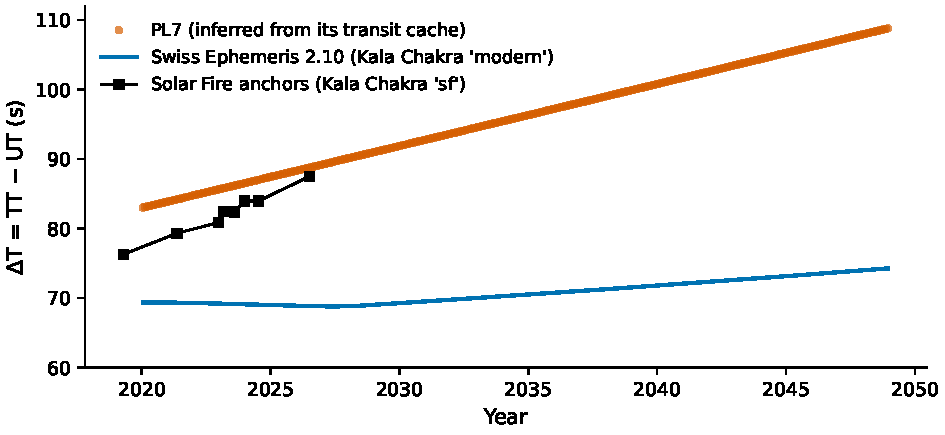
\includegraphics[width=\textwidth]{figures/fig_deltat.pdf}
  \caption[Delta-T used by PL7, Solar Fire and the Swiss Ephemeris]{\textbf{PL7 and Solar
  Fire both over-estimate $\Delta T$; PL7 by 14--20~s over 2020--2026.} \emph{What is
  shown.} Orange points: $\Delta T$ implied by PL7's cached Moon longitudes, one point per
  cached month (348 months, 2020--2048), obtained by dividing the Moon residual against the
  Swiss Ephemeris by the Moon's speed. Blue line: the Swiss Ephemeris~2.10 value used by
  Kala Chakra's \emph{modern} mode. Black squares: the eight Solar Fire anchors used by
  Kala Chakra's \emph{sf} mode (\texttt{ephemeris.js}). \emph{What to take from it.} In the
  years the family uses (2020--2026) PL7's $\Delta T$ is 1--5~s larger than Solar Fire's,
  which moves the Moon by about 1--3$''$; planets are unaffected at the arcsecond level.}
  \label{fig:deltat}
\end{figure}

\ksimple $\Delta T$ only matters for the Moon. A 5-second disagreement moves the Moon by
about $3''$, which is far below the width of a KP sub (the smallest is $40'$), so
this difference is harmless for star and sub lords.

\subsection{Ayanamsa}
\label{sec:ayanamsa}

The ayanamsa is computed in a single routine, \texttt{fcn.0055d3ea}, that is short enough
to decode completely \tagBIN. It first evaluates a Lahiri polynomial,
\begin{equation}
  A_{\text{Lahiri}} = 22^\circ 27' 37.65'' + 5026.87434''\,T + 1.11113''\,T^2,
  \qquad T = \frac{\mathrm{JD} - 2451545}{36525} + 1,
  \label{eq:lahiri}
\end{equation}
where $T$ is Julian centuries from the epoch J1900.0 (JD~2415020.0). A one-byte setting
(offset \texttt{0x67e} of the options object) then selects one of eight branches. For
branches~3--8 a second time argument is used,
\begin{equation}
  t' = \frac{\mathrm{JD} - 2415020.5}{36524},
  \label{eq:tprime}
\end{equation}
which is centuries of 36\,524 days counted from 1900~January~0.5. The widget-to-selector
mapping was recovered from the dialog constructor (\texttt{0x4c01b0}, which names each
radio button and stores it at a fixed member offset) and the OK handler
(\texttt{0x4c6ef0}, which writes the selector according to the checked button)
\tagBIN. The result is \autoref{tab:ayanamsa}. Finally the routine returns
$C - A$, where $C$ is the value typed in the ``offset'' box of the dialog
(\texttt{calculations\_offsetEdit}, default~0); sidereal longitude is tropical longitude
plus this return value.

\begin{table}[htbp]
  \centering
  \small
  \caption[PL7's eight ayanamsa options]{PL7's ayanamsa options as decoded from
  \texttt{fcn.0055d3ea}. ``Value 2025'' is at 2025~January~1 0h~UT. ``vs SE'' is PL7
  minus the Swiss Ephemeris ayanamsa of the same name (mean equinox, 2025); ``vs KC'' is
  PL7 minus Kala Chakra's effective ayanamsa (Swiss Lahiri $- 1.251''$).}
  \label{tab:ayanamsa}
  \begin{tabularx}{\textwidth}{c l >{\raggedright\arraybackslash}X r r r}
    \toprule
    Sel. & Button & Formula ($A$ in degrees) & Value 2025 & vs SE & vs KC \\
    \midrule
    1 & Lahiri (default) & \autoref{eq:lahiri} & 24°12$'$23.0$''$ & $+0.2''$ & $+1.4''$ \\
    2 & None & $0$ (tropical / sayana) & 0 & -- & -- \\
    3 & Yukteshwar & $21.015 + 1.5\,t'$ \;(54$''$/yr) & 22°53$'$24.2$''$ & $+223''$ & -- \\
    4 & Raman & $21.013888889 + 1.398148148\,t'$ & 22°45$'$41.8$''$ & $+5.7''$ & -- \\
    5 & Bhasin & $21.363888889 + 1.398148148\,t'$ & 23°06$'$41.8$''$ & n/a & -- \\
    6 & Fagan--Bradley & $23.348888889 + 1.398148148\,t'$ & 25°05$'$47.8$''$ & $+25''$ & -- \\
    7 & Krishnamurti & $22.453973785 + 1.3955235417\,t'$ & 24°11$'$54.3$''$ & $+320''$ & $-27''$ \\
    8 & Krishnamurti New & $A_{\text{Lahiri}} - 0.101388 + 0.0011118\,t'$ & 24°06$'$23.0$''$ & $-11''$ & $-359''$ \\
    \bottomrule
  \end{tabularx}
\end{table}

Three results matter for the family's work \tagNUM:

\begin{enumerate}[leftmargin=*]
  \item \textbf{PL7's Lahiri is the same Lahiri as Kala Chakra's.} Over 1900--2050 it
  agrees with the Swiss Ephemeris \texttt{SIDM\_LAHIRI} to within $0.3''$, and with Kala
  Chakra's Solar-Fire-calibrated value to $1.4''$. Lahiri charts from the two programs
  therefore agree on every star and sub lord except for points lying within $1.4''$ of a
  boundary (0.02\,\% of random longitudes).
  \item \textbf{``Krishnamurti'' (selector~7) is the classical 291~AD straight-line
  formula.} $22.453974^\circ$ at 1900 with $50.2388''$~yr$^{-1}$ is exactly zero
  ayanamsa in 291~AD at Krishnamurti's published rate of $50.2388475''$~yr$^{-1}$
  ($1609 \times 50.2388'' = 22.454^\circ$). Today it is only $27''$ smaller than Lahiri,
  and it differs from the Swiss Ephemeris's \texttt{SIDM\_KRISHNAMURTI} by about $5'20''$.
  \item \textbf{``Krishnamurti New'' (selector~8) is Lahiri minus $6'05''$} (plus a drift
  of $4''$ per century). It is within $11''$ of the Swiss Ephemeris KP ayanamsa. If a PL7
  user selects it, about 6.8\,\% of all longitudes acquire a different star or sub lord
  from the Lahiri value Kala Chakra uses (\autoref{sec:compare}).
\end{enumerate}

\begin{keybox}\kidea The family's charts are cast in Lahiri. PL7 at its default setting uses
the same Lahiri ayanamsa as Kala Chakra to within $1.4''$. The two KP options in PL7 are
genuinely different ayanamsas, and Kala Chakra offers neither.\end{keybox}

\subsection{True or mean equinox (nutation)}

With the Swiss Ephemeris's nutation switched off (\texttt{SEFLG\_NONUT}), PL7's cached
Rahu agrees with the Swiss true node minus \autoref{eq:lahiri} to $-0.54'' \pm 0.02''$ in
January~2020, and to within $\pm 0.8''$ in every month to 2048; with nutation switched on
the residual is $-16.6''$, which is exactly the nutation in longitude $\Delta\psi$ at
that date \tagNUM. PL7 therefore measures sidereal longitudes from the \emph{mean}
equinox of date. This is the same convention that the Swiss Ephemeris applies internally
in sidereal mode, so it is \emph{not} a difference from Kala Chakra.

\subsection{Rahu and Ketu: true node}

The cached Rahu matches the Swiss Ephemeris \emph{true} node to sub-arcsecond precision
and differs from the mean node by up to $1.4^\circ$ in a month \tagNUM. PL7 uses the true
node, as does Kala Chakra. Ketu is diametrically opposite.

\subsection{House cusps: Placidus, always}
\label{sec:placidus}

The chart-calculation method (code at \texttt{0x55fefc}) calls one cusp routine,
\texttt{fcn.00406c94}, unconditionally: there is no branch on any house-system setting
before the call \tagBIN. That routine carries the debug labels \texttt{plac cusp 0}
\ldots\ \texttt{plac cusp 4}. It computes the ascendant and MC, then for the intermediate
cusps calls an iterative helper (\texttt{fcn.0040684a}) with the fractions 1/3 and 2/3 and
the angular offsets $30^\circ$, $60^\circ$, $120^\circ$, $150^\circ$, using
\texttt{atan}: the textbook semi-arc trisection that defines the Placidus system
\tagBIN. The twelve cusps are written to an array at offset \texttt{0xf0}; elements~0 and~9
(cusp~1 and cusp~10) are then copied to the ascendant and MC fields. The dialog has no
house-system option; the manual's discussion of bhavas is in \autoref{sec:bhava}.

\begin{keybox}\kidea Your father was right: PL7 casts Placidus cusps. Kala Chakra casts
Topocentric (Polich--Page) cusps, which is what Solar Fire Gold was set to.\end{keybox}

\paragraph{Latitude.} The executable contains no WGS84 constant (neither
$(1-f)^2 = 0.99330562$ nor $1 - e^2$), so PL7 almost certainly feeds the \emph{geographic}
latitude to the house formula, whereas Kala Chakra converts it to \emph{geocentric}
latitude, reproducing Solar Fire's ``geocentric correction to latitude'' option \tagINF.

\paragraph{How large is the difference?} Using the Swiss Ephemeris house functions for
2000 random moments in 2019--2026, \autoref{tab:cusps} compares PL7's method (Placidus,
geographic latitude) with Kala Chakra's (Topocentric, geocentric latitude) at the two
canonical places \tagNUM. Placidus and Topocentric cusps on their own differ by only a few
arcseconds at these latitudes; almost all of the difference comes from the latitude
convention, which shifts the ascendant--descendant axis.

\begin{table}[htbp]
  \centering
  \small
  \caption[Placidus (PL7) versus Topocentric (Kala Chakra) cusps]{Absolute difference
  between PL7-style cusps (Placidus, geographic latitude) and Kala Chakra cusps
  (Topocentric, geocentric latitude), in arcseconds, over 2000 random moments in
  2019--2026. Cusps 4 and 10 coincide by construction. ``Flip'' is the share of all cusps
  whose star or sub lord differs.}
  \label{tab:cusps}
  \begin{tabular}{l rrrrrr r}
    \toprule
     & \multicolumn{6}{c}{Cusp (mean / max, $''$)} & \\
    \cmidrule(lr){2-7}
    Place & 1 \& 7 & 2 \& 8 & 3 \& 9 & 4 \& 10 & 5 \& 11 & 6 \& 12 & Flip \\
    \midrule
    Singapore ($1.28^\circ$N) & 8 / 12 & 6 / 8 & 3 / 4 & 0 / 0 & 3 / 4 & 5 / 8 & 0.1\,\% \\
    Lapanga ($21.70^\circ$N) & 149 / 227 & 126 / 209 & 71 / 122 & 0 / 0 & 70 / 122 & 125 / 209 & 1.7\,\% \\
    \bottomrule
  \end{tabular}
\end{table}

\subsection{Yogi point}
\label{sec:yogi}

\texttt{fcn.0040841f} returns $\mathrm{norm}_{360}(\lambda_\odot + \lambda_\text{Moon} +
93^\circ 20')$, using sidereal longitudes \tagBIN; the constant $93.3333\ldots$ is stored at
\texttt{0x5d1948}. This is the standard Yogi point. Its callers also compute nakshatra
indices with the helper \texttt{fcn.00566b15} (nakshatra $= 1 + \lfloor \lambda / 13^\circ
20' \rfloor$) and wrap them into $1\ldots27$; the documented definitions of Avayogi and
the Duplicate Yogi are given in \autoref{sec:yogidoc}.

% =============================================================================
\section{The transit viewer and its cache}
\label{sec:transit}
% =============================================================================

\subsection{How it works}

PL7 does not compute the transit animation from scratch each time the time step is
changed. The routines \texttt{CalcMonthEphem} and \texttt{CalcYearEphem}
(\texttt{fcn.0055dc3f}) fill a cache of planetary longitudes, one file per calendar month,
written to \texttt{Temp/YYYYM.e31} (for example \texttt{20201.e31} is January~2020). Two
check boxes in the general options, ``read transit cache'' and ``write transit cache''
(\texttt{general\_readTransitCacheCheckBox}, \texttt{general\_writeTransitCacheCheckBox}),
control whether the files are used \tagBIN. Your installation holds 436 such files covering
January~2020 to April~2056.

The file format was decoded from the data \tagNUM. Bytes 8--23 hold two doubles, the first
and last Julian Day of the month (0h~UT). From byte 840 there is one block of 64 doubles
per body, the block for body $i$ starting at byte $840 + 512\,i$, holding the sidereal
longitude every 12~hours (63 samples for a 31-day month). The body order
Sun, Moon, Mars, Mercury, Jupiter, Venus, Saturn, Rahu was identified from each series'
mean daily motion and position (for example, the first block advances $31.6^\circ$ in
January~2020, the Sun's rate, and the eighth moves retrograde by $0.6^\circ$, a node), and
confirmed by the sub-arcsecond fits below; the later blocks hold slower outer-planet series
and were not used. When you step the viewer forwards or backwards, PL7 interpolates in these
12-hour tables.

\subsection{The cache is not accurate for the planets}
\label{sec:moonvector}

Comparing the cache with the Swiss Ephemeris (Lahiri as in \autoref{eq:lahiri}, mean
equinox) shows two very different behaviours \tagNUM:

\begin{itemize}[leftmargin=*]
  \item \textbf{Moon and Rahu are right.} The Moon agrees after allowing for PL7's larger
  $\Delta T$ (\autoref{sec:deltat}); Rahu agrees to under $1''$.
  \item \textbf{Every other planet is wrong by up to about $10'$,} with an error that
  oscillates once per lunar month (\autoref{fig:moonvector}a).
\end{itemize}

The oscillation has a simple geometric cause. If a planet at geocentric distance $\Delta$
were observed not from the centre of the Earth but from a point displaced by the Moon's
geocentric vector $\vec r_{\text{Moon}}$, its longitude would shift by
\begin{equation}
  \delta\lambda \approx k\,\frac{r_{\text{Moon}}}{\Delta}\,
     \sin(\lambda_{\text{Moon}} - \lambda_{\text{planet}}),
  \label{eq:moonvector}
\end{equation}
with $k = 1$ for the full vector. Regressing each planet's residual on this predictor
explains $R^2 = 0.991$--$0.999$ of the variance, and the fitted coefficient is
$k = 0.967 \pm 0.020$ across 36 planet-months (six planets, six months spread over
2020--2045), independent of the planet's distance (\autoref{fig:moonvector}b) \tagNUM.

\begin{figure}[htbp]
  \centering
  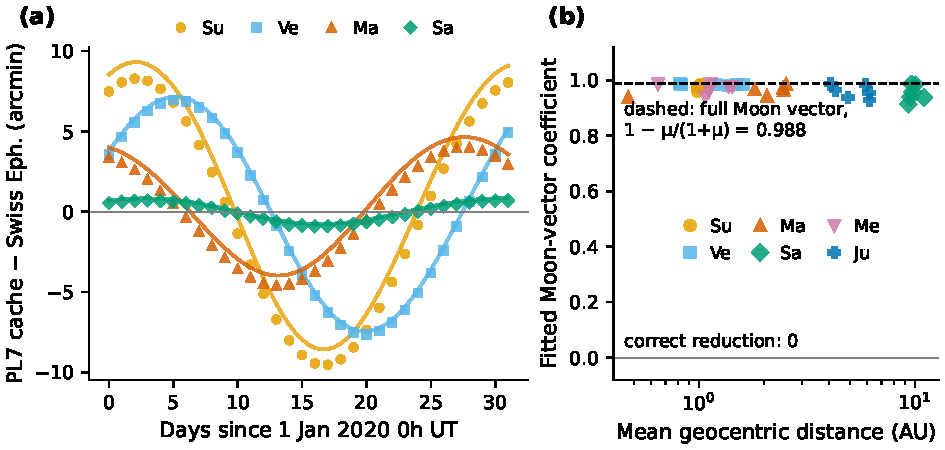
\includegraphics[width=\textwidth]{figures/fig_transit_moon_vector.pdf}
  \caption[The Moon-vector error in PL7's transit cache]{\textbf{PL7's cached planet
  positions are displaced as if seen from a point one Moon-distance away from the Earth.}
  \emph{What is shown.} (a)~Points: PL7's cached sidereal longitude minus the Swiss
  Ephemeris value (monthly mean removed) for the Sun, Venus, Mars and Saturn in January~2020,
  every day; lines: the error predicted by \autoref{eq:moonvector} with
  $k = 1 - \mu/(1+\mu) = 0.988$, no fitting. (b)~The coefficient $k$ fitted separately for
  each of six planets in six months (2020--2045), against the planet's mean geocentric
  distance on a logarithmic axis. The dashed line is the full-Moon-vector prediction; a
  correct Earth--Moon reduction would give $k=0$ (grey line). \emph{What to take from it.}
  The error is not random noise and not a low-precision ephemeris: it is one specific
  geometric mistake whose size shrinks with distance (Sun $\sim\!9'$, Saturn $\sim\!1'$)
  and which the Moon and Rahu escape.}
  \label{fig:moonvector}
\end{figure}

\subsection{Where the error comes from in the code}

Planetary series in such ephemerides are stored for the Earth--Moon barycentre (EMB). To
obtain the Earth, the Moon's geocentric vector is multiplied by $\mu/(1+\mu)$, where
$\mu = M_{\text{Moon}}/M_\oplus \approx 1/81.30$, and subtracted from the EMB. In PL7 this
reduction is in \texttt{fcn.0055e125} \tagBIN. It loads $\mu = 0.01230002$ (address
\texttt{0x5f2e28}) but does \emph{not} divide by the constant $1 + \mu$. Instead it builds
an integer $N$ at run time from four fields of the global application object (offsets
\texttt{0x91c}, \texttt{0x948}, \texttt{0x9b4}, \texttt{0x928}) and uses $\mu/(N + \mu)$:
\begin{equation}
  \text{factor} = \frac{\mu}{N + \mu} =
  \begin{cases} 0.01215 & N = 1 \text{ (correct)},\\ 1 & N = 0. \end{cases}
\end{equation}
With $N = 0$ the whole Moon vector is removed and the planets are seen from a point about
$384\,000$~km from the Earth, consistent with the measured $k = 0.967 \pm 0.020$ (theory
$0.988$). Both planet routines (all-bodies \texttt{fcn.0055ec16} and single-body
\texttt{fcn.0055e5a6}) call this reduction, and both are reached from the one dispatcher
(\texttt{fcn.0055fc12}) used for chart calculation \tagBIN.

The four fields are written mainly inside a block of about ten near-identical code
fragments (\texttt{0x583c7a}--\texttt{0x587xxx}). The PL7 \texttt{readme.txt} says that
the program shipped with a HASP hardware key. A run-time integer that should equal~1 and
silently corrupts results when it does not is a known design for licence-dependent
integrity checks. The installation analysed here was set up following instructions that
replace \texttt{PL7.exe} (\texttt{Important.png} in the \texttt{GeoVision} folder). The most
likely explanation is therefore that this copy runs without the conditions the program
expects, and computes $N = 0$ \tagINF. I did not analyse the licensing code, and the
report gives no instructions about it.

\begin{warnbox}\kpit Because the natal chart uses the same routines, the natal Sun,
Mercury, Venus, Mars, Jupiter and Saturn in \emph{this} installation are probably wrong by
up to about $10'$ as well, while the Moon, Rahu and Ketu, the ascendant and the cusps, and
therefore the Vimshottari dasha, are unaffected. This was \emph{not} directly measured,
because the saved charts (\texttt{GeoVisionCharts/*.xml}) contain only birth data. A
two-minute test is given in \autoref{sec:tests}.\end{warnbox}

\begin{qbox}\kq \emph{``Does this explain why the dasha dates matched Kala Chakra 40/40
while I distrusted the transits?''} Yes. The dasha depends only on the Moon, which this
error does not touch; the transit animation shows the planets, which it does.\end{qbox}

% =============================================================================
\section{Divisional charts (vargas)}
\label{sec:vargas}
% =============================================================================

\subsection{What PL7 offers}

The manual lists sixteen Parashari vargas (D1, D2, D3, D4, D7, D9, D10, D12, D16, D20,
D24, D27, D30, D40, D45, D60) and four Tajika vargas: Panchamsha D5, Shashtamsha D6,
Ashtamsha D8 and Ekadashamsha D11 \tagDOC\ \parencite[pp.~40, 52--53]{geovision2006pl7}. It
also mentions ``alternate'' vargas marked II or III, without defining them. PL7's own
documentation gives \emph{no} computational rule for any varga; the bundled translation of
BPHS (\texttt{CHAP/CHAP06.TXT}) states the classical rules for D9, D10 and D24 only.

\subsection{What the code actually does}

All vargas go through one dispatcher, \texttt{fcn.0057d9cf}, a 31-way \texttt{switch} on
the varga's position in the list. A byte table at \texttt{0x5f47b8} gives the divisor of
each position: $1, 2, 3, 4, 7, 9, 10, 12, 16, 20, 24, 27, 30, 40, 45, 60$ (positions
1--16), then $5, 6, 8, 11$ (the Tajika four), then $150$ (Nadiamsha), then ten alternate
vargas with divisors $2, 2, 3, 4, 10, 12, 30, 5, 16, 11$ \tagBIN. There are two kinds of
routine:

\begin{itemize}[leftmargin=*]
  \item \textbf{Cyclic.} \texttt{fcn.0057d1e1} returns $n\lambda \bmod 360^\circ$, where
  $\lambda$ is the sidereal longitude and $n$ the divisor. Counting continuously from Aries
  in this way \emph{is} the standard Parashari rule for D7, D9, D16, D20 and D27; for D9 it
  reproduces ``movable from itself, fixed from the 9th, dual from the 5th''.
  \item \textbf{Sign-dependent.} D3, D4, D10, D12, D24, D30, D40, D45, D60, D5, D6, D8,
  D11 and two alternates have their own routines, which take the sign number $s$ (Aries
  $=1$) and the degrees $d$ within the sign.
\end{itemize}

I re-implemented the routines you asked about exactly as decoded
(\texttt{scripts/pl7\_vargas.py}); \autoref{tab:vargas} gives each rule and the starting
sign for every sign.

\begin{table}[htbp]
  \centering
  \small
  \caption[Decoded varga rules]{Varga rules decoded from \texttt{PL7.exe} \tagBIN.
  ``Start'' is the sign of the first amsa for Aries, Taurus, Gemini \ldots\ Pisces, taken
  from the re-implementation. $s$ = sign number (Aries $=1$); $d$ = degrees in the sign.}
  \label{tab:vargas}
  \begin{tabularx}{\textwidth}{>{\raggedright\arraybackslash}p{2.5cm} l >{\raggedright\arraybackslash}X >{\raggedright\arraybackslash}p{3.7cm}}
    \toprule
    Varga & Routine & Rule & Start (Ar \ldots Pi) \\
    \midrule
    D9 Navamsha & \texttt{0057d1e1} & $9\lambda \bmod 360$ (cyclic from Aries) & Ar Cp Li Cn, repeating \\
    D10 Dashamsha & \texttt{0057d55c} & odd $s$: from the sign itself; even $s$: from the 9th & Ar Cp Ge Pi Le Ta Li Cn Sg Vi Aq Sc \\
    D24 Chatur\-vimshamsha & \texttt{0057d675} & odd $s$: from Leo; even $s$: from Cancer & Le Cn, repeating \\
    D6 Shashtamsha & \texttt{0057d4dc} & odd $s$: from Aries; even $s$: from Libra & Ar Li, repeating \\
    D8 Ashtamsha & \texttt{0057d510} & movable: from Aries; fixed: from Sagittarius; dual: from Leo & Ar Sg Le, repeating \\
    D11 Ekadashamsha & \texttt{0057d5a6} & $(11d/30 + 1 - s)\times 30$, identical to $11\lambda \bmod 360$ (cyclic from Aries) & Ar Pi Aq Cp Sg Sc Li Vi Le Cn Ge Ta \\
    D11 alternate (position 31) & \texttt{0057d5d6} & $(1 - 11d/30)\times 30$: every sign starts at Aries and counts \emph{backwards} & Ar for all (2nd amsa Pi) \\
    D16 alternate (position 30) & \texttt{0057d5fb} & odd $s$: forwards from the sign; even $s$: backwards & Ar Le Ge Li Le Sg \ldots \\
    \bottomrule
  \end{tabularx}
\end{table}

\begin{notebox}\ksimple On D11: PL7 has two Ekadashamsha rules and no rule named
Rudramsha or ``Iyer''. Its main D11 is the plain continuous count from Aries; its alternate
D11 counts backwards from Aries for every sign. If the ``Iyer'' D11 you have in mind is a
third rule, PL7 does not implement it, and Kala Chakra has no D11 at all. Given the rule,
it can be added to Kala Chakra as a single function.\end{notebox}

Varga strength (Vimshopaka) is offered on 6-, 7-, 10- and 16-varga schemes with scores of
5--20, and the planetary table's ``vimshopaka bala'' column uses the 10-varga scheme
\tagDOC\ \parencite[p.~145]{geovision2006pl7}. The per-varga weights are not documented and
were not decoded.

% =============================================================================
\section{Bhava chalit (the Bhava chart)}
\label{sec:bhava}
% =============================================================================

PL7 does not use the name ``Bhava Chalit''; the equivalent is the \emph{Bhava chart}
\tagDOC. Three house divisions are offered as special charts
\parencite[p.~56]{geovision2006pl7}:

\begin{enumerate}[leftmargin=*]
  \item \textbf{Bhava (Sripati)}, centred on the ascendant. The tutorial
  (\texttt{Extras1/pib11770}) defines it: the ascendant and MC are the madhyas (centres) of
  houses 1 and 10 and the opposite points those of 7 and 4; ``the spaces in between are
  further divided in 3 equal portions''; and ``the Bhava Sandhis are placed halfway between
  each pair of adjacent houses''. This is Porphyry-style trisection of each quadrant,
  applied to bhava \emph{centres}.
  \item \textbf{Bhava (equal)}: each house spans $15^\circ$ either side of a madhya set by
  the ascendant degree.
  \item \textbf{Krishnamurti chart (Placidus)}, in which the ascendant is the
  \emph{beginning} of the first house; this is the KP cusp chart of \autoref{sec:placidus}.
\end{enumerate}

\begin{keybox}\kidea PL7's ``bhava chalit'' is a Sripati chart: \emph{centres} at Asc and MC
with quadrant trisection. Kala Chakra's houses are KP-style \emph{beginnings}
(Topocentric cusps). The two answer different questions, so a planet can legitimately sit
in different houses in the two programs even with identical longitudes.\end{keybox}

% =============================================================================
\section{Yogi, Avayogi and Duplicate Yogi}
\label{sec:yogidoc}
% =============================================================================

The manual never states the Yogi formula; the binary does (\autoref{sec:yogi}): the Yogi
point is Sun $+$ Moon $+$ $93^\circ 20'$ \tagBIN. The report templates print ``Yogi
Point'', ``Yogi'' (the lord of the Yogi point's nakshatra) and a combined field
``Avayogi/Duplicate Yogi'' (\texttt{Extras1/pib337}) \tagDOC. The dictionary defines
Avayogi only as the point opposite the Yogi point \parencite[p.~208]{geovision2006pl7};
the Duplicate Yogi is not defined at all. Definitions of both vary between authors, and PL7's documentation does not say which it
uses; I could not settle them from the code within the time available, so they are left
open here rather than filled in from general knowledge. Kala Chakra computes
none of these points.

% =============================================================================
\section{Dashas}
\label{sec:dashas}
% =============================================================================

\subsection{Systems and levels}

PL7 offers at least twenty dasha systems (Vimshottari, Ashtottari, Shodashottari,
Dwadashottari, Panchottari, Shatabdika, Chaturashitisama, Dwisaptatisama, Shastihayani,
Shattrimshatsama, Kalachakra, Chara, Sthira, Niryana Shoola, Drig, Yogini, Navamsha,
Tribhagi, Tribhagi~40, Narayana, and more below the visible part of the list), shown to at
most five levels: maha, antar, pratyantar, sookshma and prana \tagDOC\
\parencite[pp.~42--44]{geovision2006pl7}. The reference body can be the Moon (default), the
ascendant or any planet. The balance at birth is computed ``by degree'' (fraction of
$13^\circ 20'$ traversed, the default) or ``by time''. Kala Chakra computes Vimshottari only,
but to \emph{six} levels (adding deha), by degree from the Moon, anchored once at the chart
moment.

\subsection{The dasha year: a hidden discrepancy}

The Dashas tab offers ``360 days or 365.25 days or 327.85 days for a dasha year'', and its
screenshot shows 365.25 selected \tagDOC\ \parencite[pp.~193--194]{geovision2006pl7}. The
code says something different \tagBIN. The OK handler (\texttt{0x4c7dc2}) writes setting byte
\texttt{0x68c}: 2 for the ``360'' button, 1 for ``365.25'' and 3 for ``327.85''; the
reset-to-defaults routine also sets~1. The year-length function \texttt{fcn.00464743} then
returns 360.0 for~2 and 327.85 for~3, but for~1 it returns \emph{365.2421875} days (the
tropical year), not 365.25. The Vimshottari start is computed as birth minus year length
times balance (\texttt{fcn.00460018}), and the year-length function is called from six places in
the dasha routines (\texttt{0x4600e8}, \texttt{0x4601af}, \texttt{0x460600}, \texttt{0x460697},
\texttt{0x4606b9}, \texttt{0x4709b4}). The constant 365.25 does occur in the same code region, but
next to 30.6001, 122.1, 1524 and 1\,720\,994.5: the Meeus calendar-to-Julian-Day conversion, not
a dasha year. Your PL7 dasha screenshots used for the 40/40 check (RA Job, SG, MANTA) show
periods within about two years of the chart, consistent with the explanation below.

\begin{derivbox}
\textbf{Why the 40/40 validation could not see this.} The two year lengths differ by
$0.0078$~day, or $11.25$~minutes per year of dasha time. Your validation compared dates
near the chart moment, within about $\pm 5$ years, so the boundaries moved by under an hour
and fell on the same calendar date. For a natal chart the drift grows: about $1.9$~h at 10
years from birth and about $11$~h at 60 years, which is enough to move pratyantar and
sookshma boundaries by a day, and prana boundaries much more.
\end{derivbox}

For horary use, where the periods of interest lie within weeks of the chart, the two
programs agree. If exact PL7 parity is ever wanted for long-range natal dashas, Kala Chakra
would need 365.2421875-day years. Either way, the knowledge base's description of the PL7
convention as ``365.25-day years'' should be corrected.

% =============================================================================
\section{The KP section: calculation and display}
\label{sec:kp}
% =============================================================================

\textbf{Cusps.} Placidus, with the cusp as the beginning of the house \tagBIN\ \tagDOC\
\parencite[pp.~56, 200]{geovision2006pl7}.

\textbf{Ayanamsa.} The dictionary says KP printouts use the Krishnamurti ayanamsa
``regardless of the default set'' \parencite[pp.~218--219]{geovision2006pl7}. In the code,
the only places that write the values 7 or 8 to the ayanamsa selector are in the options
dialog. Two printing/model routines (\texttt{fcn.00553970}, \texttt{fcn.00578e80}) load the
selector from a stored record (field \texttt{+0x260}), which matches the manual's
per-astrologer ayanamsa setting for model printing \parencite[p.~165]{geovision2006pl7}.
Which KP ayanamsa (selector 7 or 8) a KP printout uses was \emph{not determined} \tagINF.

\textbf{Lords.} The planetary and cusp tables show the nakshatra lord and sub lord
\parencite[p.~145]{geovision2006pl7}. Sub-sub lords are not documented and no sub-sub
column exists \tagDOC.

\textbf{Display.} PL7 has a circular KP chart, whose ``inner ring shows the Rashis, the next
ring the Nakshatras, the next the houses'' \parencite[p.~200]{geovision2006pl7}, with a table
of sub lords, occupants, ``tenants'' (planets in the nakshatras of occupants), owner and
tenants of the owner. There are also four KP worksheets (Krishnamurti, Krishnamurti~II,
Krishnamurti Prashna, Krishnamurti Prashna~II) and two reports. ``KP -- Chart'' gives the
birth chart, cuspal chart and ``Bhava Details (Placidus System)''. ``KP -- Significators''
gives the houses signified by planets, graded from ``very strong significator'' down; ruling
planets (day lord, lagna sign/star/sub lord, Moon sign/star/sub lord); and Fortuna \tagDOC.

\textbf{Horary.} ``Krishnamurti Prashna'' is cast for the current time ``and the ascendant
is based on a number selected by the user'' (worksheet help). Two integer-input calls in the
binary are bounded at 249 (\texttt{0x553f5a}, \texttt{0x557a21}), so the number is almost
certainly 1--249 \tagINF. The number-to-ascendant table was not decoded.

\begin{keybox}\kidea For KP horary, Kala Chakra is ahead of PL7 in four concrete ways. It
gives a five-level sub-lord chain (PL7 stops at the sub). It computes the family's
cusp-number vectors and power calculation, which PL7 has no notion of. It replicates Solar
Fire to $\le 1''$. And it is not affected by the Moon-vector planet error of
\autoref{sec:moonvector}. PL7 is ahead in breadth: significator grading, ruling planets,
Fortuna, and 1--249 horary ascendants.\end{keybox}

% =============================================================================
\section{Jaimini: karakas, padas and special lagnas}
\label{sec:jaimini}
% =============================================================================

Jaimini is implemented in PL7 \tagDOC. Everything below comes from the documentation; none
of it exists in Kala Chakra.

\textbf{Chara karakas.} A calculation option chooses 8 karakas including Rahu or 7 without
\parencite[p.~192]{geovision2006pl7}. Separately, the worksheet offers ``Karakas(8)'' and
``Karakas(7)'', where the 7-karaka scheme merges the mother and children karakas. Rahu's
degree is measured backwards (30 minus its degree in the sign). The default is not
documented.

\textbf{Aspects.} Rashi drishti: ``fixed signs aspect all the movable signs except the one
next to it'', and vice versa; dual signs aspect each other
\parencite[pp.~216--217]{geovision2006pl7}.

\textbf{Arudha padas.} A ``Jaimini padas and lagnas'' worksheet shows the padas of all twelve
houses for the birth chart, Navamsha and Dashamsha. The rule is to count from the house to
its lord, then as many houses again \parencite[p.~222]{geovision2006pl7}. The exceptions are
stated two different ways:

\begin{itemize}[leftmargin=*]
  \item The tutorial (\texttt{pib11755}): lord in the 4th or 7th gives the 4th house as
  Arudha Lagna, and lord in the 1st gives the 10th.
  \item The bundled BPHS (\texttt{CHAP29}): a pada falling in the same house goes to the
  10th from it, and one falling in the 7th goes to the 4th from the original house.
\end{itemize}

\textbf{The two disagree when the lord is in the 7th}, and neither says which the engine
applies \tagDOC.

\textbf{Upapada.} ``Generally considered as the pada of the 12th house, though there are
different views'' \parencite[p.~230]{geovision2006pl7}.

\textbf{Karakamsha and Swamsha.} Both are offered; the Karakamsha chart ``takes the sign of
the Atma Karaka (AK) in the Navamsha as the ascendant'', drawn on the birth chart or on the
Navamsha \parencite[p.~57]{geovision2006pl7}.

\textbf{Special lagnas.} Bhava lagna advances $15^\circ$ per hour from the Sun's position at
sunrise, Hora lagna one sign per hour, and Ghatika lagna one sign per 24 minutes; Varnada,
Indu and Pranapada are also given. Sunrise is taken at the Sun's edge or its centre, as an
option \parencite[p.~192]{geovision2006pl7}; the default and the refraction handling are not
documented.

\textbf{Argala.} Planets in the 2nd, 4th, 11th and 5th from a point cause argala, obstructed
from the 12th, 10th, 3rd and 9th; the direction is reversed for Rahu and Ketu.

% =============================================================================
\section{Guna matching (compatibility)}
\label{sec:guna}
% =============================================================================

PL7 offers both systems \tagDOC\ \parencite[pp.~104--106]{geovision2006pl7}:

\begin{itemize}[leftmargin=*]
  \item \textbf{Ashtakoota} (North Indian), on the Moon's nakshatra: varna, vashya, tara,
  yoni, graha maitri, gana, bhakoot and nadi, totalling 36. Gana, bhakoot and nadi are
  flagged as \emph{maha doshas}, and the Pancha-nadi exception is mentioned. The points per
  koota are not stated in any readable line.
  \item \textbf{Dashakoota} (South Indian, after Kalaprakasika), with three totals printed
  (Kalaprakasika, B.~V.~Raman and Ashtakoota methods): ``a number below 18 is questionable,
  between 18 and 24 is good and above 24 is excellent''.
  \item \textbf{Manglik (Kuja) dosha}: Mars in the 1st, 2nd, 4th, 7th, 8th or 12th from the
  ascendant and from the Moon, with seven printed cancellation rules.
  \item Matching can also be run on planets other than the Moon, and a rashi-distance
  comparison is offered.
\end{itemize}

There are no options to configure the koota rules. Kala Chakra has no matching module.

\Needspace{8\baselineskip}
% =============================================================================
\section{The planetary ``summariser'' table}
\label{sec:summary}
% =============================================================================

The planetary-details table has fifteen selectable columns \tagDOC\
\parencite[p.~145]{geovision2006pl7}: degrees; retrograde/combust flag; sign; nakshatra;
pada; nakshatra lord/sub; dignity; shadbala; vimshopaka bala (10 vargas); varga
classification; avasthas in the 3-, 5-, 9- and 12-state schemes; and lordships. The cusp
table has degrees, sign, nakshatra, pada and nakshatra lord/sub.

Kala Chakra's tables show degree, star lord and the five-level sub chain, house placement,
ownership numbers and the power string. They have no retrograde flag (the engine requests
no planetary speed), no dignity, no shadbala, no vimshopaka and no avasthas.

% =============================================================================
\section{Side by side: PL7 and Kala Chakra 1.5}
\label{sec:compare}
% =============================================================================

Kala Chakra~1.5 here means the single-file app \texttt{Kala Chakra v1.5.html} (and its
sibling \texttt{KAAST Caster v1.5.html}) in \texttt{Advanced\_Setup/web/dist/}. Its casting
engine is \texttt{Advanced\_Setup/web/src/ephemeris.js}, \texttt{kp\_logic.js} and
\texttt{dasha.js}; I checked that the dist files contain these sources byte for byte.
\autoref{tab:compare} sets the two engines side by side.

\begin{table}[htbp]
  \centering
  \footnotesize
  \caption[PL7 versus Kala Chakra 1.5]{The two casting engines compared. Grades refer to the
  PL7 column; the Kala Chakra column is from its source code.}
  \label{tab:compare}
  \begin{tabularx}{\textwidth}{>{\raggedright\arraybackslash}p{2.5cm} >{\raggedright\arraybackslash}X >{\raggedright\arraybackslash}X}
    \toprule
    Item & Parashara's Light 7.0 & Kala Chakra 1.5 \\
    \midrule
    Ephemeris & Own files (\texttt{ephemdat.bin}, \texttt{topos*.dat}), J2000 equatorial; precise to end of 2048, coarse fallback after \tagNUM & Swiss Ephemeris 2.10.03 (WASM), files 1800--2399 \\
    $\Delta T$ & 1993 table, extrapolated: 83~s (2020) to 109~s (2048) \tagNUM & Solar Fire anchors 76--88~s (\emph{sf}) or Swiss $\approx 69$~s (\emph{modern}) \\
    Ayanamsa & 8 options; default Lahiri $=$ Swiss Lahiri $\pm 0.3''$; two KP variants \tagBIN & Lahiri only, Swiss $- 1.251''$ (Solar Fire clone) \\
    Equinox & Mean equinox of date \tagNUM & Mean equinox of date (Swiss sidereal mode) \\
    Node & True (in this installation; true/mean option exists) \tagNUM & True \\
    Planet positions & Geocentric; in this copy displaced by $\approx 0.97\times$ the Moon vector (up to $\sim\!10'$) \tagNUM & Geocentric apparent, $\le 1''$ from Solar Fire \\
    House cusps & Placidus, geographic latitude \tagBIN/\tagINF & Topocentric, geocentric (WGS84) latitude \\
    Bhava chart & Sripati (centres, quadrant trisection) and equal \tagDOC & Not offered (houses are KP beginnings) \\
    Rounding & Not determined & Truncated to whole arcseconds \\
    Star/sub lords & Star and sub \tagDOC & Star plus five-level sub chain \\
    KP extras & Significators, ruling planets, Fortuna, horary 1--249 \tagDOC/\tagINF & Cusp-number vectors, span rule, power calculation \\
    Vargas & 16 Parashari $+$ 4 Tajika $+$ D150 $+$ 10 alternates \tagBIN & None \\
    Yogi points & Yogi $=$ Sun $+$ Moon $+ 93^\circ 20'$ \tagBIN & None \\
    Dashas & $\ge 20$ systems, 5 levels; ``365.25'' option actually 365.2421875~d \tagBIN & Vimshottari, 6 levels, 365.25~d \\
    Jaimini \& padas & Karakas (7/8), rashi drishti, arudhas, upapada, special lagnas, argala \tagDOC & None \\
    Transit viewer & Animated circle, steps 1~s to 10~yr, via a 12-hourly month cache \tagBIN/\tagNUM & None (one chart per cast) \\
    Guna matching & Ashtakoota, Dashakoota, Manglik \tagDOC & None \\
    \bottomrule
  \end{tabularx}
\end{table}

\subsection{What the differences do to star and sub lords}

A KP sub is at least $40'$ wide (the Sun's sub, $13^\circ 20' \times 6/120$), so a difference
matters only for points lying within that difference of a boundary. Using random longitudes and the cusp
simulation of \autoref{tab:cusps} \tagNUM:

\begin{itemize}[leftmargin=*]
  \item PL7 Lahiri vs Kala Chakra Lahiri ($1.4''$): 0.02\,\% of points change star or sub
  lord.
  \item PL7 ``Krishnamurti'' vs Kala Chakra ($27''$): 0.5\,\%.
  \item PL7 ``Krishnamurti New'' vs Kala Chakra ($5'59''$): 6.8\,\%.
  \item Placidus with geographic latitude vs Topocentric with geocentric latitude: 0.1\,\%
  of cusps at Singapore and 1.7\,\% at Lapanga.
  \item The Moon-vector error ($\sim\!1'$--$10'$) in this PL7 copy: for an error of
  about $8'$ against an average sub width of $89'$, roughly one Sun, Mercury or Venus position
  in ten gets a different sub lord; the Moon and the nodes are unaffected.
\end{itemize}

\begin{keybox}\kidea For the family's KP horary work the casting engines differ in three
choices, Lahiri versus KP ayanamsa, Placidus versus Topocentric, and the latitude
convention, plus one defect specific to this PL7 copy. Kala Chakra's choices were made
deliberately to replicate the Solar Fire profile the family uses, and they are validated
against the family's own hand-calculated charts. That validation, not either program, is
the authority for the method.\end{keybox}

% =============================================================================
\section{Tests you can run in PL7 yourself}
\label{sec:tests}
% =============================================================================

These take a few minutes each and settle the points this report could only infer.

\begin{enumerate}[leftmargin=*]
  \item \textbf{Is this copy's Sun wrong?} Cast one chart in PL7 with Lahiri, say for
  1~January~2020 at 0:00~UT (5:30~IST) at any place, and read the Sun to the second.
  Cast the same moment in KAAST Caster in \emph{modern} mode, which gives about
  $255^\circ 52' 40''$ (Sagittarius $15^\circ 52' 40''$). PL7's own transit cache holds
  $256^\circ 01' 09''$ for that instant, $8'29''$ larger. If PL7's chart shows the larger value,
  the Moon-vector error is present in natal charts too. The Moon should agree to about $10''$
  (PL7's larger $\Delta T$ accounts for about $7''$).
  \item \textbf{Which KP ayanamsa does the KP printout use?} Set the Calculation tab to
  Lahiri, print the Krishnamurti chart, and read the ``KP Ayanamsha'' line. Compare with
  \autoref{tab:ayanamsa}: about $24^\circ 11' 54''$ (Krishnamurti) or $24^\circ 06' 23''$
  (Krishnamurti New) at 1~January~2025.
  \item \textbf{Rahu true or mean.} In Options $\to$ Calculation $\to$ Miscellaneous, check
  the ``Rahu \& Ketu'' item; the cache says \emph{true} in this installation.
  \item \textbf{D11.} Display the Ekadashamsha and its alternate (II/III) version for a
  planet at Taurus $1^\circ$: the main D11 should put it in Pisces, the alternate in Aries.
\end{enumerate}


% =============================================================================
\section{Limitations}
\label{sec:limits}
% =============================================================================

PL7 was never run. Everything about its numerical behaviour comes from the transit cache,
which covers 2020--2056 and holds planets and nodes but not cusps. The cusp comparison of
\autoref{tab:cusps} is therefore a simulation of PL7's method with the Swiss Ephemeris house
functions, not a measurement of PL7's own cusps. The claim that PL7 uses geographic
latitude rests on the absence of the WGS84 constants. The statement that the Moon-vector
error also affects natal charts rests on shared code paths, not on a measured natal chart.
The link between that error and the licence state is an inference from the code structure
and the installation notes; the licensing code itself was deliberately not analysed.

Without a decompiler, routines were read from x87 disassembly. The short routines
(ayanamsa, vargas, Yogi point, dasha year, Earth--Moon factor) were decoded in full; the
Placidus routine was identified by its structure, its debug labels and its constants rather
than traced instruction by instruction. The ephemeris data files were not decoded, so the
underlying theory (VSOP, a JPL development or other) and the lower date limit are unknown.
Where the manual and the code disagree (dasha year) or the manual is silent (D6, D8, D11,
Yogi), this report follows the code. Where neither was conclusive (Avayogi, Duplicate Yogi,
arudha exceptions, which KP ayanamsa the KP printout forces, chara-karaka default), the
report says so instead of filling the gap from general astrological knowledge.

% =============================================================================
\section*{AI Tool Declaration}
\addcontentsline{toc}{section}{AI Tool Declaration}
% =============================================================================

This report was prepared with Claude (Anthropic) running in Claude Code, which performed
the binary analysis through REA and Rizin, wrote and ran the numerical scripts, and drafted
the text. A sub-agent read the PL7 documentation; every page citation was checked against
the extracted manual text. The conclusions should be read with the evidence grades in mind.

\printbibliography[heading=bibintoc, title={References}]

\appendix
% =============================================================================
\section{Key addresses in \texttt{PL7.exe}}
\label{app:addresses}
% =============================================================================

\begin{longtable}{>{\raggedright\arraybackslash\ttfamily}p{4.3cm} >{\raggedright\arraybackslash}p{10.9cm}}
  \toprule
  \normalfont Address & Role \\
  \midrule
  \endhead
  0x55d3ea & Ayanamsa: Lahiri polynomial plus 8-way selector (byte \texttt{+0x67e}), user offset (\texttt{+0x250}) \\
  0x4c01b0 / 0x4c6ef0 & Calculation dialog: radio-button construction / OK handler writing the selector \\
  0x5682d6 & Reset to defaults: selector $=1$ (Lahiri), offset $=0$, dasha year byte $=1$ \\
  0x405cc3, 0x5822cb & Temporary switch to tropical (selector 2) for sayana quantities \\
  0x55fefc & Chart method: calls the cusp routine unconditionally, copies Asc and MC \\
  0x406c94 & Placidus cusps (``plac cusp'' labels, semi-arc trisection helper 0x40684a) \\
  0x55de40 & Ephemeris reader (\texttt{EQU2000} frame, date-range check) \\
  0x55e125 & Earth--Moon reduction; factor $\mu/(N+\mu)$ with run-time $N$ \\
  0x55ec16 / 0x55e5a6 & All-planets / single-planet position routines \\
  0x55fc12 & Dispatcher for planet calculation \\
  0x55dc3f & \texttt{CalcMonthEphem} / \texttt{CalcYearEphem} (transit cache) \\
  0x40841f & Yogi point: Sun $+$ Moon $+ 93^\circ 20'$ \\
  0x464743 & Dasha year length: 360 / 327.85 / 365.2421875 days \\
  0x460018 & Vimshottari start epoch from the balance \\
  0x57d9cf & Varga dispatcher (31 cases); divisor table at 0x5f47b8 \\
  0x57d1e1 & Cyclic varga $n\lambda \bmod 360$ \\
  0x57d55c, 0x57d675, 0x57d4dc, 0x57d510, 0x57d5a6 & D10, D24, D6, D8, D11 respectively \\
  0x57d5d6, 0x57d5fb & Alternate D11, alternate D16 \\
  0x553f5a, 0x557a21 & Integer inputs bounded at 249 (KP horary number) \\
  \bottomrule
\end{longtable}

% =============================================================================
\section{Citation provenance}
\label{app:provenance}
% =============================================================================

{\setlength{\tabcolsep}{4pt}% Auto-generated by render_provenance.py — do not edit by hand
\begin{landscape}
\scriptsize
\begin{longtable}{p{0.0920\linewidth}p{0.1380\linewidth}p{0.0644\linewidth}p{0.1380\linewidth}p{0.1656\linewidth}p{0.0644\linewidth}p{0.0644\linewidth}p{0.0828\linewidth}p{0.0644\linewidth}}
\caption{Citation provenance ledger: every reference, where it was accessed, what was read, the claim it supports and the supporting passage in the source.}\label{tab:provenance}\\
\toprule
\textbf{Key} & \textbf{Reference} & \textbf{Cited where} & \textbf{Claim in manuscript} & \textbf{What the source says (as read)} & \textbf{Location} & \textbf{Accessed from} & \textbf{Read} & \textbf{Status} \\
\midrule
\endfirsthead
\toprule
\textbf{Key} & \textbf{Reference} & \textbf{Cited where} & \textbf{Claim in manuscript} & \textbf{What the source says (as read)} & \textbf{Location} & \textbf{Accessed from} & \textbf{Read} & \textbf{Status} \\
\midrule
\endhead
\midrule\multicolumn{9}{r}{\emph{continued on next page}}\\
\endfoot
\bottomrule
\endlastfoot
\texttt{geovision\allowbreak{}2006\allowbreak{}pl\allowbreak{}7} & GeoVision / Parashara Software (2006). Parashara's Light 7.0 User's Manual (English PL 7 Manual, 3 March 2006). Bundled as PL7/PL70.pdf. & Vargas §: list & PL7 lists sixteen Parashari vargas & ``There are sixteen Vargas (divisional charts), including the birth chart.'' & p. 40 & user-supplied-pdf & FULL+\allowbreak{}FIG & VERIFIED \\
\texttt{geovision\allowbreak{}2006\allowbreak{}pl\allowbreak{}7} & GeoVision / Parashara Software (2006). Parashara's Light 7.0 User's Manual (English PL 7 Manual, 3 March 2006). Bundled as PL7/PL70.pdf. & Vargas §: Tajika & Four Tajika vargas D5, D6, D8, D11 & ``The Tajika Vargas are the Panchamsha (1/5 division of a sign), the Shashtiamsha (1/6 division), Ashtamsha (1/8 division) and Ekadashamsha (1/11 division of a sign).'' & pp. 52-53 & user-supplied-pdf & FULL+\allowbreak{}FIG & VERIFIED \\
\texttt{geovision\allowbreak{}2006\allowbreak{}pl\allowbreak{}7} & GeoVision / Parashara Software (2006). Parashara's Light 7.0 User's Manual (English PL 7 Manual, 3 March 2006). Bundled as PL7/PL70.pdf. & Vargas §: vimshopaka & Vimshopaka column uses 10 vargas & ``vimshopaka bala gives the vimshopaka strength for a group of 10 vargas'' & p. 145 & user-supplied-pdf & FULL+\allowbreak{}FIG & VERIFIED \\
\texttt{geovision\allowbreak{}2006\allowbreak{}pl\allowbreak{}7} & GeoVision / Parashara Software (2006). Parashara's Light 7.0 User's Manual (English PL 7 Manual, 3 March 2006). Bundled as PL7/PL70.pdf. & Bhava § & Three house divisions: Sripati, equal, Krishnamurti (Placidus); Sripati centred on Asc, KP begins at Asc & ``The ‘Krishnamurti Chart’ is based on the Placidious system of calculation of houses. The Bhava (Sripati) and Bhava (equal) charts treat the ascendant as the center of the first house.'' & p. 56 & user-supplied-pdf & FULL+\allowbreak{}FIG & VERIFIED \\
\texttt{geovision\allowbreak{}2006\allowbreak{}pl\allowbreak{}7} & GeoVision / Parashara Software (2006). Parashara's Light 7.0 User's Manual (English PL 7 Manual, 3 March 2006). Bundled as PL7/PL70.pdf. & Yogi § & Avayogi defined only as the point opposite the Yogi point & ``Ava Yogi : The point opposite the Yogi point that has an effect on a person’s wealth.'' & p. 208 (Dictionary) & user-supplied-pdf & FULL+\allowbreak{}FIG & VERIFIED \\
\texttt{geovision\allowbreak{}2006\allowbreak{}pl\allowbreak{}7} & GeoVision / Parashara Software (2006). Parashara's Light 7.0 User's Manual (English PL 7 Manual, 3 March 2006). Bundled as PL7/PL70.pdf. & Dashas §: levels & At most five dasha levels; default display four & ``You can see at most 5 levels at once (Prana dashas).'' & p. 42 & user-supplied-pdf & FULL+\allowbreak{}FIG & VERIFIED \\
\texttt{geovision\allowbreak{}2006\allowbreak{}pl\allowbreak{}7} & GeoVision / Parashara Software (2006). Parashara's Light 7.0 User's Manual (English PL 7 Manual, 3 March 2006). Bundled as PL7/PL70.pdf. & Dashas §: year & UI offers 360, 365.25, 327.85-day dasha years & ``Dasha Year : Choose to use either 360 days or 365.25 days or 327.85 days for a dasha year.'' & p. 193 & user-supplied-pdf & FULL+\allowbreak{}FIG & VERIFIED \\
\texttt{geovision\allowbreak{}2006\allowbreak{}pl\allowbreak{}7} & GeoVision / Parashara Software (2006). Parashara's Light 7.0 User's Manual (English PL 7 Manual, 3 March 2006). Bundled as PL7/PL70.pdf. & KP §: ayanamsa & KP printouts force the Krishnamurti ayanamsa & ``Krishnamurti printouts use the Krishnamurti ayanamsha regardless of the default set'' & pp. 218-219 (Dictionary) & user-supplied-pdf & FULL+\allowbreak{}FIG & VERIFIED \\
\texttt{geovision\allowbreak{}2006\allowbreak{}pl\allowbreak{}7} & GeoVision / Parashara Software (2006). Parashara's Light 7.0 User's Manual (English PL 7 Manual, 3 March 2006). Bundled as PL7/PL70.pdf. & KP §: per-astrologer settings & Model printing stores a preferred ayanamsa per astrologer & ``Select the prefered ‘Ayanamsha’. Also select between true and mean Rahu and the desired chart style.'' & p. 165 & user-supplied-pdf & FULL+\allowbreak{}FIG & VERIFIED \\
\texttt{geovision\allowbreak{}2006\allowbreak{}pl\allowbreak{}7} & GeoVision / Parashara Software (2006). Parashara's Light 7.0 User's Manual (English PL 7 Manual, 3 March 2006). Bundled as PL7/PL70.pdf. & KP §: lords & Tables show nakshatra lord and sub lord & ``nakshatra lord/sub gives the lord(ruler) of the nakshatra and the sublord'' & p. 145 & user-supplied-pdf & FULL+\allowbreak{}FIG & VERIFIED \\
\texttt{geovision\allowbreak{}2006\allowbreak{}pl\allowbreak{}7} & GeoVision / Parashara Software (2006). Parashara's Light 7.0 User's Manual (English PL 7 Manual, 3 March 2006). Bundled as PL7/PL70.pdf. & KP §: display & Circular KP chart with rashi, nakshatra and house rings & ``The inner ring shows the Rashis, the next ring the Nakshatras, the next the houses with their numbers inside.'' & p. 200 & user-supplied-pdf & FULL+\allowbreak{}FIG & VERIFIED \\
\texttt{geovision\allowbreak{}2006\allowbreak{}pl\allowbreak{}7} & GeoVision / Parashara Software (2006). Parashara's Light 7.0 User's Manual (English PL 7 Manual, 3 March 2006). Bundled as PL7/PL70.pdf. & Jaimini §: karakas & 8 karakas with Rahu or 7 without & ``Select Rahu too, to use 8 karakas, including Rahu. Select No Rahu to use just 7 karakas.'' & p. 192 & user-supplied-pdf & FULL+\allowbreak{}FIG & VERIFIED \\
\texttt{geovision\allowbreak{}2006\allowbreak{}pl\allowbreak{}7} & GeoVision / Parashara Software (2006). Parashara's Light 7.0 User's Manual (English PL 7 Manual, 3 March 2006). Bundled as PL7/PL70.pdf. & Jaimini §: aspects & Rashi drishti rule & ``Fixed signs aspect all the movable signs except the one next to it.'' & pp. 216-217 (Dictionary) & user-supplied-pdf & FULL+\allowbreak{}FIG & VERIFIED \\
\texttt{geovision\allowbreak{}2006\allowbreak{}pl\allowbreak{}7} & GeoVision / Parashara Software (2006). Parashara's Light 7.0 User's Manual (English PL 7 Manual, 3 March 2006). Bundled as PL7/PL70.pdf. & Jaimini §: padas & Pada counting rule & ``Counting as many houses away from a house lord as the house lord is away from it’s house gives the pada of a house.'' & p. 222 (Dictionary) & user-supplied-pdf & FULL+\allowbreak{}FIG & VERIFIED \\
\texttt{geovision\allowbreak{}2006\allowbreak{}pl\allowbreak{}7} & GeoVision / Parashara Software (2006). Parashara's Light 7.0 User's Manual (English PL 7 Manual, 3 March 2006). Bundled as PL7/PL70.pdf. & Jaimini §: upapada & Upapada is generally the pada of the 12th & ``It is generally considered as the pada of the 12th house, though there are different views as to it’s correct calculation.'' & p. 230 (Dictionary) & user-supplied-pdf & FULL+\allowbreak{}FIG & VERIFIED \\
\texttt{geovision\allowbreak{}2006\allowbreak{}pl\allowbreak{}7} & GeoVision / Parashara Software (2006). Parashara's Light 7.0 User's Manual (English PL 7 Manual, 3 March 2006). Bundled as PL7/PL70.pdf. & Jaimini §: Karakamsha & Karakamsha in birth chart and in Navamsha & ``The Karakamsha chart takes the sign of the Atma Karaka (AK) in the Navamsha as the ascendant for the Karakamsha chart.'' & p. 57 & user-supplied-pdf & FULL+\allowbreak{}FIG & VERIFIED \\
\texttt{geovision\allowbreak{}2006\allowbreak{}pl\allowbreak{}7} & GeoVision / Parashara Software (2006). Parashara's Light 7.0 User's Manual (English PL 7 Manual, 3 March 2006). Bundled as PL7/PL70.pdf. & Guna § & Dashakoota score bands & ``A number below 18 is questionable, between 18 and 24 is good and above 24 is excellent.'' & p. 106 & user-supplied-pdf & FULL+\allowbreak{}FIG & VERIFIED \\
\texttt{geovision\allowbreak{}2006\allowbreak{}pl\allowbreak{}7} & GeoVision / Parashara Software (2006). Parashara's Light 7.0 User's Manual (English PL 7 Manual, 3 March 2006). Bundled as PL7/PL70.pdf. & Engine §: Lahiri default & Lahiri is the default ayanamsa & ``By default the Lahiri Ayanamsha is used.'' & p. 190 & user-supplied-pdf & FULL+\allowbreak{}FIG & VERIFIED \\
\texttt{geovision\allowbreak{}2006\allowbreak{}pl\allowbreak{}7} & GeoVision / Parashara Software (2006). Parashara's Light 7.0 User's Manual (English PL 7 Manual, 3 March 2006). Bundled as PL7/PL70.pdf. & Jaimini §: sunrise option & Sunrise from limb or centre is an option & ``Some people use the edge of the Sun for this calculation, and others use the exact, astronomical longitude of the Sun.'' & p. 192 & user-supplied-pdf & FULL+\allowbreak{}FIG & VERIFIED \\
\texttt{morluto\allowbreak{}2026\allowbreak{}rea} & morluto (2026). REA: Reverse Engineer Anything. GitHub repository and rea-agents npm package v6.5.0. & Methods § & REA connects an agent to native-binary analysis engines and returns evidence records & ``REA connects your agent to tools for inspecting native binaries, JavaScript and Electron apps, .NET assemblies, and websites.'' & README (repository main, cloned 2026-10-17) & publisher-direct & FULL\_TEXT & VERIFIED \\
\end{longtable}
\end{landscape}
}

\end{document}
